% Entrega A8 — Manuscrito científico (SPEC-000 §11.4; SPEC-009)
% Experimento oficial: exp-a4-v2
% Toda afirmação quantitativa rastreável a results/ e article/tables|figures (DOC-R03).
\documentclass[11pt,a4paper]{article}

\usepackage[margin=2.5cm]{geometry}
\usepackage{fontspec}
\usepackage{graphicx}
\usepackage{booktabs}
\usepackage{tabularx}
\usepackage{hyperref}
\usepackage{xcolor}
\usepackage{caption}
\usepackage{subcaption}
\usepackage{amsmath}
\usepackage{microtype}
\usepackage{csquotes}
\usepackage[backend=biber,style=numeric,sorting=none]{biblatex}
\addbibresource{references.bib}

\setmainfont{DejaVu Serif}
\setsansfont{DejaVu Sans}
\setmonofont{DejaVu Sans Mono}

\hypersetup{
  colorlinks=true,
  linkcolor=blue!50!black,
  citecolor=blue!50!black,
  urlcolor=blue!60!black
}

\graphicspath{{../figures/}}

\title{Benchmark reproduzível de métodos clássicos de aprendizado de máquina\\
para diagnóstico de falhas no Tennessee Eastman Process}
\author{Grupo A --- WP1A / MEI0028 --- Modelagem e Simulação\\
\textit{Pontifícia Universidade Católica de Goiás}}
\date{2026-09-14}

\begin{document}
\maketitle

\begin{abstract}
Este artigo apresenta um benchmark reproduzível de seis famílias clássicas de
aprendizado de máquina --- regressão logística, árvore de decisão, random forest,
gradient boosting, SVM e XGBoost --- para diagnóstico multiclasse de falhas no
Tennessee Eastman Process (TEP). O protocolo fixa a execução do processo
(\texttt{run}) como unidade de divisão e de análise, exige o mesmo manifesto e
o mesmo pré-processamento para todos os modelos, isola o conjunto de teste até o
congelamento das configurações e avalia desempenho e custo de forma multicritério.
No experimento oficial \texttt{exp-a4-v2}, random forest, XGBoost e gradient
boosting lideram as métricas globais no teste; regressão logística e SVM linear
formam o grupo inferior. O líder em acurácia (XGBoost, 0,618) não coincide com o
líder em F1 macro e MCC (random forest, 0,357 e 0,597). Entre classes presentes
no holdout, as falhas 3, 15 e 10 são as de menor F1 médio; as confusões 10$\to$15
e 3$\to$15 são as mais frequentes. Pelos critérios binários de SPEC-000~\S4
no holdout, H1--H4 são \emph{corroboradas}. Em nível de execução (SPEC-008;
acurácia por \texttt{run}, $n{=}11$), Friedman rejeita igualdade global
($p{=}0{,}015$); Wilcoxon+Holm na família H1 corrobora ensembles${>}$LR, enquanto
a família H2 não corrobora RF/XGB${>}$DT. Ameaças estruturais incluem
cobertura disjunta de classes entre validação e teste (dois \texttt{runs} por
classe no dataset canônico), semente/split únicos e orçamentos de busca
desiguais. O benchmark destina-se a servir de referência clássica
para estudos futuros com modelos profundos, físico-informados ou de detecção precoce.
\end{abstract}

\tableofcontents
\newpage

%==============================================================================
\section{Introdução}
\label{sec:intro}
%==============================================================================

O diagnóstico automático de falhas em processos químicos industriais exige
mapear variáveis de processo a condições operacionais (normal versus modos de
falha) com protocolo experimental transparente. Comparações entre classificadores
frequentemente misturam partições inconsistentes, permitem vazamento temporal
entre treino e teste e concluem ``melhor modelo'' apenas por acurácia simples ---
métrica frágil sob desbalanceamento entre classes~\cite{chiang2001fault,yin2012tep}.

O Tennessee Eastman Process (TEP)~\cite{downs1993tep} é um ambiente simulado de
referência com 52 variáveis de processo e 21 classes (condição normal e 20
falhas). Este trabalho desenvolve um \textbf{benchmark reproduzível} de seis
famílias clássicas de aprendizado de máquina sob um único protocolo, respondendo
a cinco questões de pesquisa (QP1--QP5) e avaliando quatro hipóteses (H1--H4).

\paragraph{Contribuições.}
(i)~protocolo anti-vazamento com divisão agrupada por execução;
(ii)~avaliação conjunta de desempenho e custo computacional (proibição de ranking
por métrica única);
(iii)~artefatos versionados (manifesto, predições, métricas, figuras) que
permitem recomputar qualquer número reportado;
(iv)~respostas explícitas a QP1--QP5 e vereditos binários (corroborada/refutada)
de H1--H4, com evidência §4 no holdout e testes SPEC-008 em nível de
\texttt{run\_id}.

\paragraph{Questões de pesquisa.}
\begin{description}
  \item[QP1] Quais algoritmos apresentam o melhor desempenho global?
  \item[QP2] O desempenho é consistente sob equilíbrio entre classes?
  \item[QP3] Quais falhas são sistematicamente mais difíceis?
  \item[QP4] Métodos mais complexos justificam maior custo?
  \item[QP5] Qual o melhor compromisso desempenho $\times$ tempo $\times$ tamanho?
\end{description}

\paragraph{Hipóteses.}
\begin{description}
  \item[H1] Conjuntos baseados em árvores superam regressão logística em F1
  macro e/ou MCC.
  \item[H2] XGBoost e random forest superam regressão logística e árvore isolada
  em F1 e MCC.
  \item[H3] Regressão logística permanece competitiva em custo, com F1 reduzido
  nas falhas difíceis.
  \item[H4] O melhor modelo por acurácia não coincide com o melhor por F1, MCC
  ou custo de inferência.
\end{description}

%==============================================================================
\section{Fundamentação sobre diagnóstico de falhas e TEP}
\label{sec:fundamentacao}
%==============================================================================

\subsection{Diagnóstico de falhas orientado a dados}

Métodos clássicos de monitoramento e diagnóstico (PCA dinâmico, CVA, PLS e
variantes) exploram correlação entre variáveis para detecção e, em alguns casos,
isolamento de falhas~\cite{russell2000fault,chiang2001fault}. Abordagens de
aprendizado supervisionado tratam o problema como classificação multiclasse:
cada observação recebe um rótulo de condição operacional. A qualidade da
conclusão depende criticamente da unidade amostral usada na divisão e nos testes
estatísticos.

\subsection{Tennessee Eastman Process}

O TEP~\cite{downs1993tep} simula uma planta com reator, condensador, separador,
stripper e reciclo. Cada execução (\emph{run}) induz (ou não) uma falha e gera
uma série temporal de observações. No presente estudo, a tarefa é classificar
vetores de 52 variáveis em uma de 21 classes. A \textbf{unidade experimental} é
a execução, não a linha individual: observações do mesmo \texttt{run} são
temporalmente correlacionadas e não podem ser tratadas como amostras
independentes na divisão nem nos testes de hipótese (INV-09; UE-03).

\subsection{Avaliação multicritério}

Em cenários com 21 classes e desbalanceamento, acurácia simples pode mascarar
fracasso em falhas minoritárias. Adotamos o conjunto de métricas globais
(acurácia, acurácia balanceada, precisão/revocação/F1 macro, F1 ponderada, MCC),
métricas por classe, matrizes de confusão e custos (tempo de treino, tempo de
inferência, tamanho do modelo). Nenhuma conclusão de superioridade se apoia
apenas em acurácia~\cite{matthews1975mcc}.

%==============================================================================
\section{Trabalhos relacionados}
\label{sec:related}
%==============================================================================

Yin et~al.~\cite{yin2012tep} comparam métodos data-driven no TEP e evidenciam a
sensibilidade dos resultados ao protocolo. Conjuntos de dados derivados do TEP
ampliaram o uso em detecção de anomalias~\cite{rieth2017tep}. Ensembles de
árvores~\cite{breiman2001rf} e boosting escalável~\cite{chen2016xgboost}, bem
como SVMs~\cite{cortes1995svm}, são famílias clássicas recorrentes em
classificação tabular.

O presente trabalho diferencia-se por: (1)~fixar a execução como unidade de
divisão com verificação automatizada de disjunção; (2)~obrigar o mesmo pipeline
para seis modelos; (3)~isolar o teste até o congelamento; (4)~reportar custo
sempre que se discute ``melhor modelo''; (5)~delimitar explicitamente o escopo
aos métodos clássicos, como referência para estudos futuros com redes profundas
ou modelos físico-informados --- fora do escopo deste benchmark.

%==============================================================================
\section{Materiais e métodos}
\label{sec:metodos}
%==============================================================================

\subsection{Dataset canônico}

Utilizamos a versão canônica \texttt{tep-canonical-v1}: 52 atributos, 21
classes, 42 execuções e 30\,260 linhas (Tabela~\ref{tab:dataset};
Figura~\ref{fig:dataset}). A auditoria prévia do pacote bruto e o registro
canônico precedem qualquer modelagem.

\begin{table}[ht]
\centering
\caption{Sumário do dataset canônico (artefato A6;
\texttt{article/tables/A6\_exp-a4-v2\_\_01\_dataset\_summary.csv}).}
\label{tab:dataset}
\begin{tabular}{lr}
\toprule
Item & Valor \\
\midrule
Features & 52 \\
Classes & 21 \\
Runs & 42 \\
Linhas & 30\,260 \\
Versão & \texttt{tep-canonical-v1} \\
\bottomrule
\end{tabular}
\end{table}

\begin{figure}[ht]
\centering
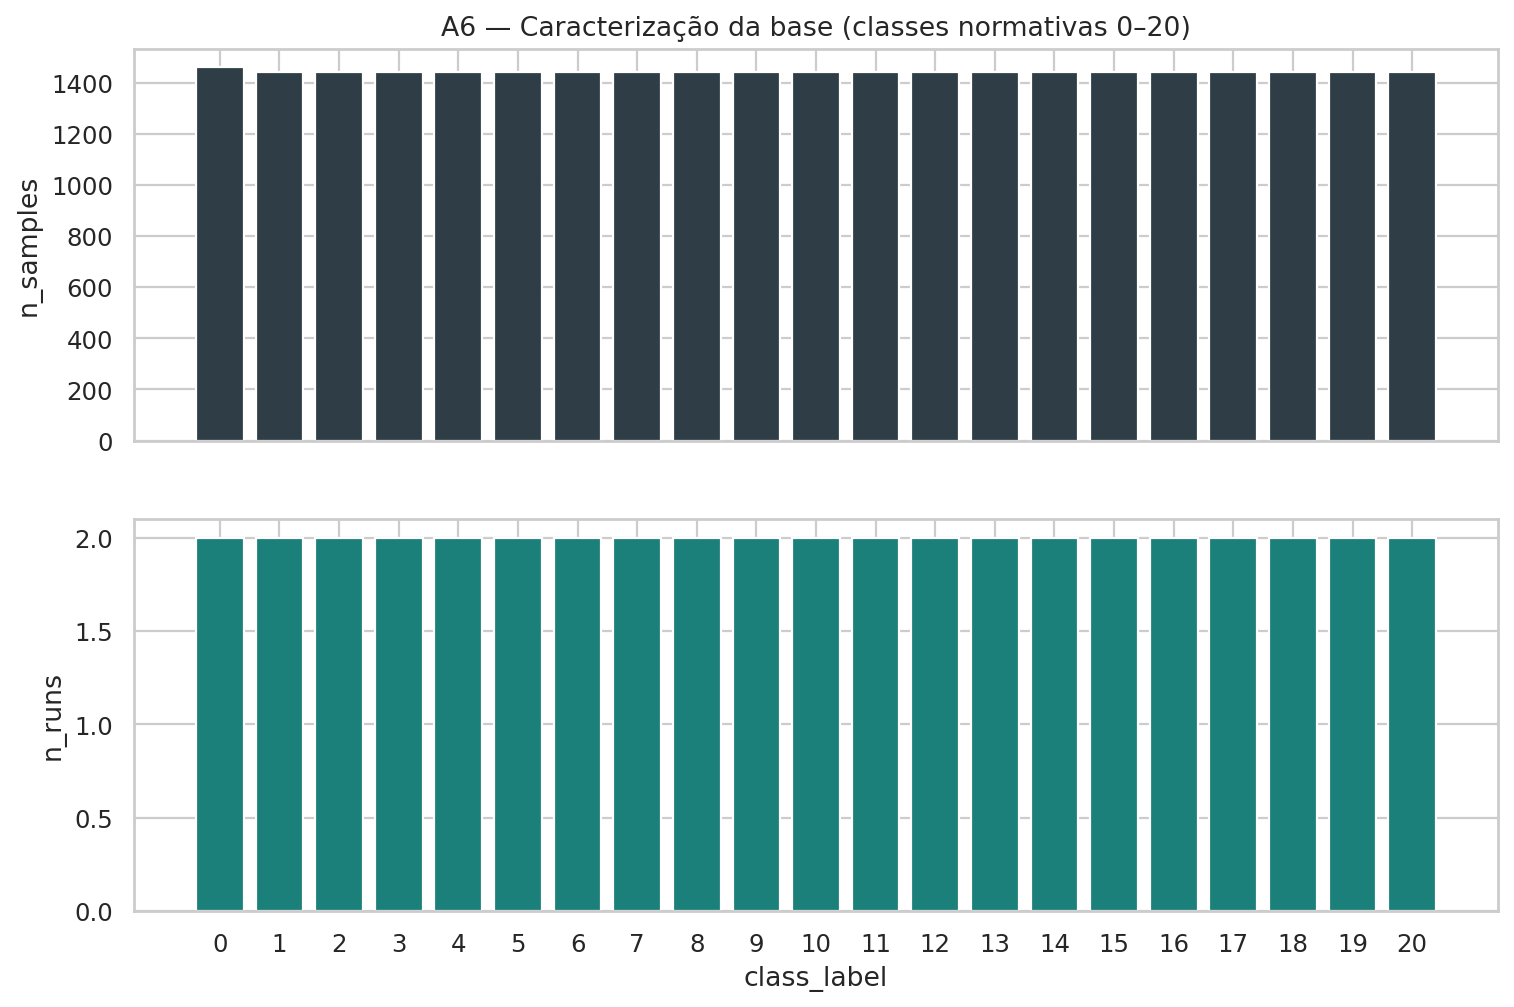
\includegraphics[width=0.85\textwidth]{A6_exp-a4-v2__01_dataset_characterization.png}
\caption{Caracterização do dataset (A6). Fonte:
\texttt{results/} via gerador A6 (sem leitura de \texttt{data/raw}).}
\label{fig:dataset}
\end{figure}

\subsection{Divisão agrupada por execução}

A estratégia \texttt{stratified\_one\_train\_per\_class\_remaining\_split\_val\_test}
reserva um \texttt{run} por classe ao treino e divide o restante aproximadamente
50/50 entre validação e teste (semente 42). Resultado: 21 runs de treino, 10 de
validação e 11 de teste. A checagem de interseção vazia de \texttt{run\_id}
passou no manifesto A3.

\paragraph{Limitação estrutural.}
Com apenas dois \texttt{runs} por classe, validação e teste \textbf{não cobrem
simultaneamente as 21 classes}. Neste experimento, os conjuntos de classes de
validação e de teste são disjuntos (validação: classes 0, 1, 4, 5, 7, 8, 9, 12,
16, 17; teste: 2, 3, 6, 10, 11, 13, 14, 15, 18, 19, 20). Essa limitação é
discutida na Seção~\ref{sec:ameacas}.

\subsection{Pré-processamento}

A versão \texttt{preprocessor\_v1} ajusta transformações dependentes dos dados
(padronização) \textbf{exclusivamente no treino} e apenas aplica
(\texttt{transform}) validação e teste.

\subsection{Modelos}

Seis classificadores sob o mesmo manifesto e o mesmo pré-processamento
(implementação via \texttt{scikit-learn}~\cite{pedregosa2011sklearn} e
XGBoost~\cite{chen2016xgboost}):

\begin{enumerate}
  \item Regressão logística (MOD-1)
  \item Árvore de decisão (MOD-2)
  \item Random forest (MOD-3)~\cite{breiman2001rf}
  \item Gradient boosting sklearn (MOD-4)
  \item SVM linear (MOD-5)~\cite{cortes1995svm}
  \item XGBoost (MOD-6)~\cite{chen2016xgboost}
\end{enumerate}

\subsection{Seleção de hiperparâmetros}

A busca usa apenas treino/validação. Os espaços desta baseline
(\texttt{exp-a4-v2}) são reduzidos e \textbf{desiguais} entre famílias (p.ex.\
gradient boosting com dois candidatos; SVM restrito a kernel linear; XGBoost com
oito candidatos). Hiperparâmetros congelados: Tabela~\ref{tab:hp}.

\begin{table}[ht]
\centering
\caption{Hiperparâmetros finais (A6;
\texttt{A6\_exp-a4-v2\_\_02\_hyperparameters.csv}).}
\label{tab:hp}
\small
\begin{tabular}{ll}
\toprule
Modelo & Parâmetros principais \\
\midrule
Regressão logística & $C{=}10$, \texttt{lbfgs}, \texttt{max\_iter}${=}1000$ \\
Árvore de decisão & \texttt{max\_depth}${=}20$, \texttt{min\_samples\_leaf}${=}5$ \\
Random forest & $n{=}200$, \texttt{max\_depth}${=}20$ \\
Gradient boosting & $n{=}50$, $\eta{=}0{,}1$, \texttt{max\_depth}${=}3$ \\
SVM & $C{=}10$, kernel linear \\
XGBoost & $n{=}100$, $\eta{=}0{,}1$, \texttt{max\_depth}${=}6$, \texttt{hist} \\
\bottomrule
\end{tabular}
\end{table}

\subsection{Métricas}

Reportamos MET-01 a MET-12. F1 macro e acurácia balanceada usam $C{=}21$:
classes ausentes no teste entram com contribuição nula e deprimem essas métricas
em relação à acurácia. Verificação formal das definições:
\texttt{formula\_checks\_ok=True} nos seis modelos
(\texttt{results/tables/A5\_exp-a4-v2\_\_global\_metrics.csv}).

%==============================================================================
\section{Protocolo reprodutível}
\label{sec:protocolo}
%==============================================================================

O pipeline segue a ordem fixa: auditoria $\to$ análise exploratória $\to$
divisão $\to$ pré-processamento $\to$ treinamento/seleção $\to$ avaliação final.
O experimento oficial é \texttt{exp-a4-v2} (substitui \texttt{exp-a4-v1},
abortado por custo no gradient boosting).

\begin{itemize}
  \item Semente: 42 (\texttt{configs/seeds.yaml}).
  \item Manifesto: \texttt{data/processed/split\_manifest\_v1.json}.
  \item Configuração: \texttt{configs/experiments/exp-a4-v2.yaml}.
  \item Snapshot de ambiente: Python 3.12.7, scikit-learn 1.9.1, XGBoost 2.1.4
  (\texttt{results/metadata/exp-a4-v2\_\_config\_snapshot.json}).
  \item SHA de execução A4: \texttt{40c6c6026f39\ldots}\ (\texttt{git\_dirty:
  true} no snapshot).
  \item Predições e métricas brutas em \texttt{results/}; figuras/tabelas de
  publicação em \texttt{article/} (geradas somente a partir de \texttt{results/}).
\end{itemize}

Um \emph{dry-run} com fração de runs existe para fumaça de pipeline e está
marcado como não científico (\texttt{scientific\_validity: false}); não alimenta
este manuscrito. Tuning ampliado (SPEC-006A) não foi executado nesta baseline.

%==============================================================================
\section{Resultados}
\label{sec:resultados}
%==============================================================================

Todos os números abaixo provêm de
\texttt{results/tables/A5\_exp-a4-v2\_\_*.csv} e das figuras A6
correspondentes.

\subsection{Desempenho global e custo}

A Tabela~\ref{tab:global} e as Figuras~\ref{fig:f1mcc}--\ref{fig:cost}
resumem o teste.

\begin{table}[ht]
\centering
\caption{Métricas globais e custo no conjunto de teste
(\texttt{A5\_exp-a4-v2\_\_global\_metrics.csv}).}
\label{tab:global}
\small
\begin{tabular}{lrrrrrrr}
\toprule
Modelo & Acc & BA & F1$_m$ & MCC & Treino\,s & Inf.\,s & Bytes \\
\midrule
Reg.\ logística & 0,275 & 0,164 & 0,184 & 0,250 & 3,65 & 0,003 & 10\,020 \\
Árvore & 0,564 & 0,303 & 0,314 & 0,560 & 1,36 & 0,0015 & 158\,662 \\
Random forest & 0,617 & \textbf{0,333} & \textbf{0,357} & \textbf{0,597} & 3,09 & 0,243 & 49\,567\,094 \\
Grad.\ boosting & 0,608 & 0,321 & 0,347 & 0,584 & 281,89 & 0,101 & 1\,901\,442 \\
SVM linear & 0,237 & 0,150 & 0,163 & 0,215 & 177,03 & 3,575 & 8\,782\,836 \\
XGBoost & \textbf{0,618} & 0,330 & 0,353 & 0,596 & 22,28 & 0,052 & 4\,910\,294 \\
\bottomrule
\end{tabular}
\end{table}

\begin{figure}[ht]
\centering
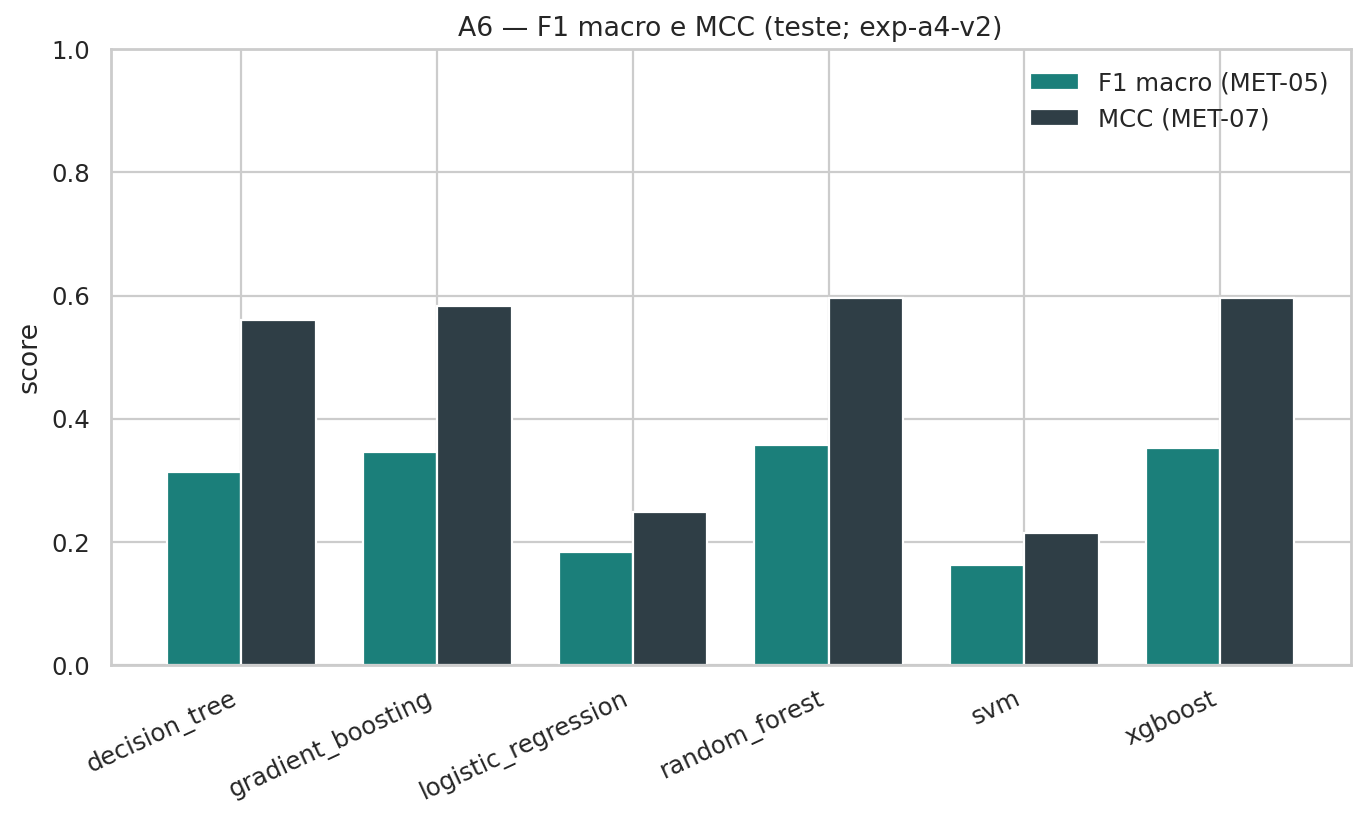
\includegraphics[width=0.9\textwidth]{A6_exp-a4-v2__06_f1_mcc.png}
\caption{Comparativo de F1 macro e MCC (A6).}
\label{fig:f1mcc}
\end{figure}

\begin{figure}[ht]
\centering
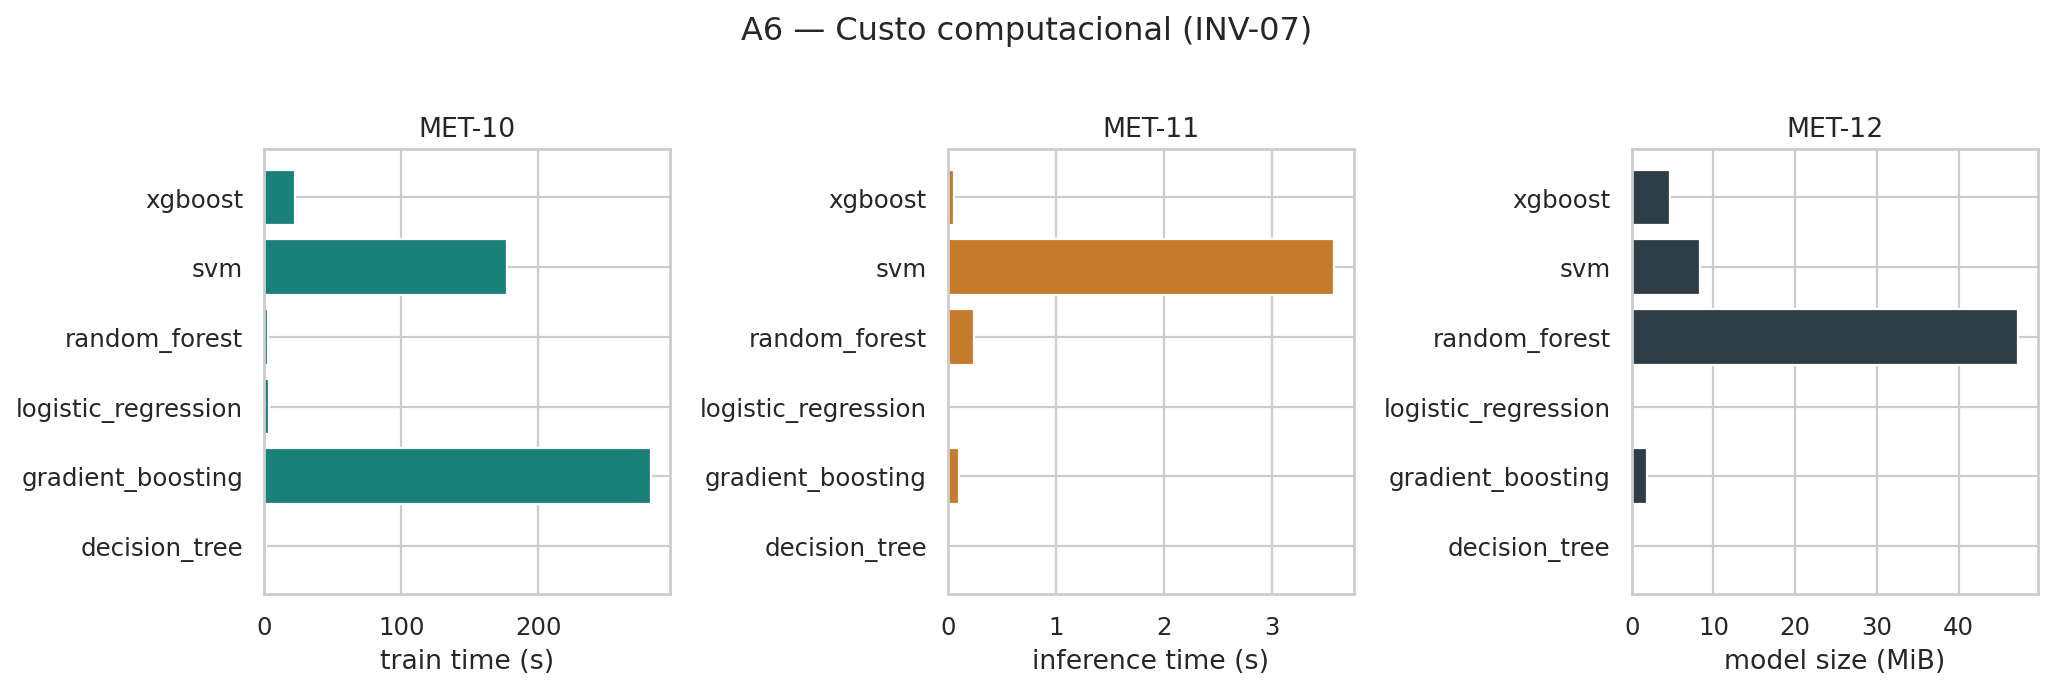
\includegraphics[width=0.9\textwidth]{A6_exp-a4-v2__07_computational_cost.png}
\caption{Custo computacional: treino, inferência e tamanho (A6).}
\label{fig:cost}
\end{figure}

\subsection{QP1 --- Desempenho global}

Os conjuntos baseados em árvores (RF, XGBoost, GB) e, em seguida, a árvore
isolada dominam as métricas globais; regressão logística e SVM linear formam o
grupo inferior. Por acurácia lidera XGBoost (0,618); por F1 macro e MCC lidera
random forest (0,357 e 0,597). Não há ranking oficial por métrica única.

\subsection{QP2 --- Equilíbrio entre classes}

O ranking por acurácia (XGB $\to$ RF $\to$ GB $\to$ DT $\to$ LR $\to$ SVM)
\textbf{não} coincide com o ranking por BA/F1/MCC (RF $\to$ XGB $\to$ \ldots).
A diferença XGB--RF é pequena, mas suficiente para afirmar inconsistência parcial
entre critérios. A lacuna acurácia $\gg$ BA/F1 é compatível com a média sobre
21 classes incluindo 10 ausentes no teste.

\subsection{QP3 --- Falhas difíceis}

Entre classes com \texttt{support}$>0$, os menores F1 médios (seis modelos)
ocorrem nas falhas \textbf{3} (0,184), \textbf{15} (0,252) e \textbf{10}
(0,283). Pares mais frequentes (soma entre modelos): 10$\to$15 (1451),
3$\to$15 (1002), 18$\to$5 (1001), 13$\to$12 (809)
(Figuras~\ref{fig:pairs}--\ref{fig:heatmap};
\texttt{A5\_exp-a4-v2\_\_qp3\_confused\_faults.json}). Classes com
\texttt{support}${=}0$ não são interpretadas como ``difíceis observadas'' neste
holdout. Não atribuímos mecanismo físico a essas confusões.

\begin{figure}[ht]
\centering
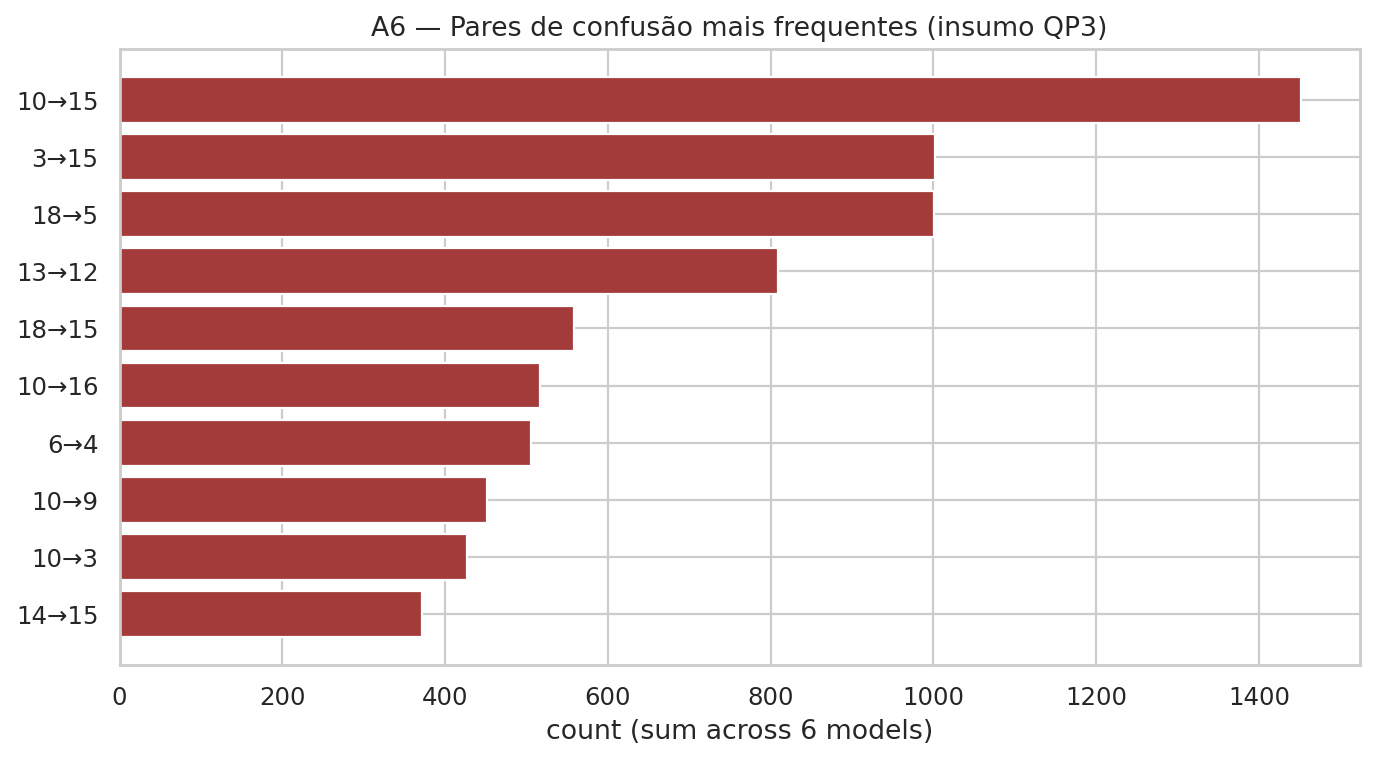
\includegraphics[width=0.85\textwidth]{A6_exp-a4-v2__08_confused_pairs.png}
\caption{Pares de confusão mais frequentes (A6).}
\label{fig:pairs}
\end{figure}

\begin{figure}[ht]
\centering
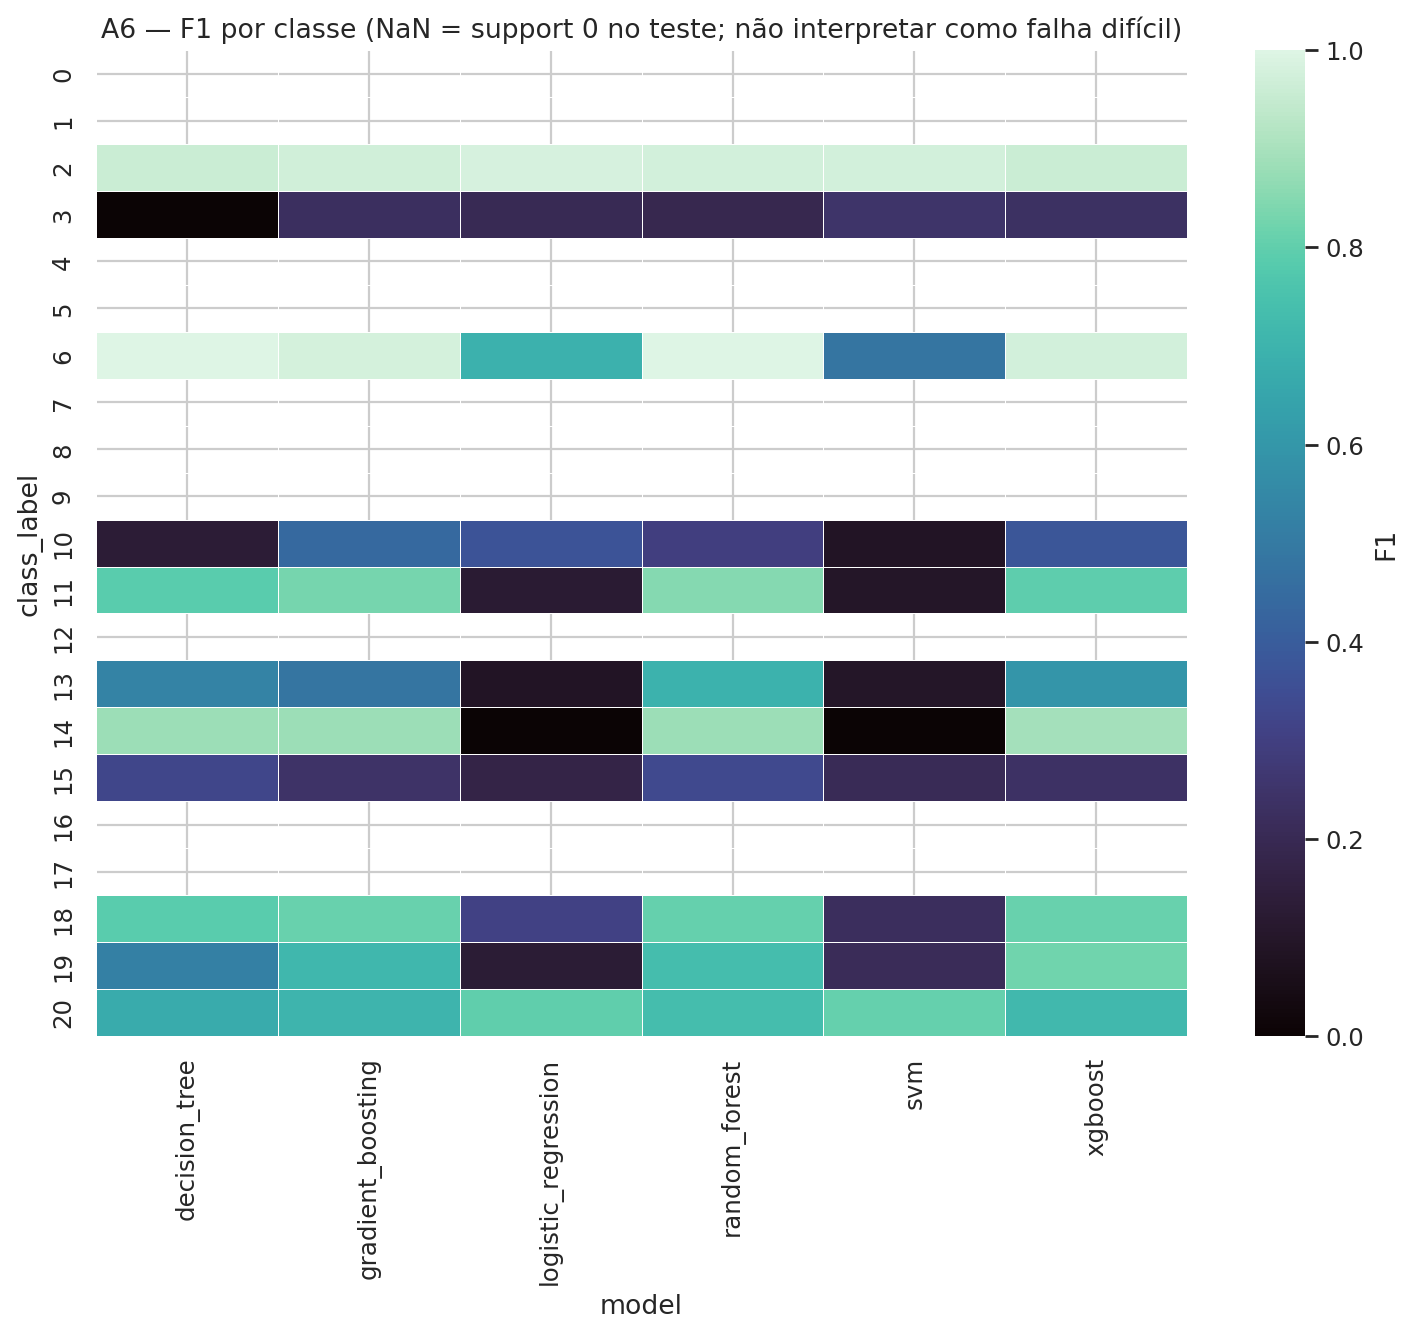
\includegraphics[width=0.95\textwidth]{A6_exp-a4-v2__08_per_class_f1_heatmap.png}
\caption{Heatmap de F1 por classe (NaN onde \texttt{support}${=}0$) (A6).}
\label{fig:heatmap}
\end{figure}

Matrizes de confusão por modelo estão em
\texttt{article/figures/A6\_exp-a4-v2\_\_05\_cm\_\_*.png}.

\subsection{QP4 --- Complexidade versus custo}

RF obtém o melhor F1/MCC com treino baixo, porém o maior artefato. XGBoost quase
empata RF com inferência mais rápida e tamanho cerca de $10\times$ menor. GB não
supera RF/XGB e tem o maior tempo de treino ($\approx$282\,s): o ganho observado
não justifica esse custo nesta baseline. SVM linear combina custo alto e pior
desempenho preditivo.

\subsection{QP5 --- Compromisso multicritério}

\begin{itemize}
  \item Maximizar F1/MCC: \textbf{random forest}.
  \item Compromisso desempenho/custo: \textbf{XGBoost}.
  \item Extremo barato com desempenho intermediário: \textbf{árvore de decisão}.
  \item Extremo compacto com desempenho global baixo: \textbf{regressão logística}.
\end{itemize}

\subsection{Análise estatística (SPEC-008)}

Unidade experimental: \texttt{run\_id}; $n{=}11$ runs de teste; métrica pareada:
acurácia dentro do run (\texttt{run\_accuracy}). Fonte:
\texttt{results/tables/A8\_exp-a4-v2\_\_*} e
\texttt{results/metrics/A8\_exp-a4-v2\_\_statistics.json}.

Friedman (6 modelos): $\chi^2{=}14{,}079$, $p{=}0{,}015$ --- rejeita igualdade
global de ranks. Médias de \texttt{run\_accuracy}: RF $0{,}635$, XGB $0{,}630$,
GB $0{,}614$, DT $0{,}579$, LR $0{,}313$, SVM $0{,}287$.

Wilcoxon com Holm \emph{dentro} de cada família planejada: H1 (3 pares
RF/GB/XGB vs LR) --- todos significativos; H2 (4 pares RF/XGB vs LR/DT) ---
\textbf{nenhum} dos quatro pares permanece significativo após Holm (incluindo
RF/XGB vs LR nesta família de tamanho 4, ao contrário da família H1 de tamanho
3; as diferenças médias vs DT são as menores). Poder limitado por $n{=}11$.
Limitação: uma semente e um split (EST-01 entre sementes não aplicável).

\subsection{Avaliação de H1--H4}

\begin{description}
  \item[H1] RF, GB e XGB superam LR em F1/MCC globais (\S4).
  \textbf{Corroborada} (§4). Run-level: \textbf{corroborada}
  (Wilcoxon+Holm, família H1).
  \item[H2] RF e XGB superam LR e DT em F1/MCC globais (\S4).
  \textbf{Corroborada} (§4). Run-level: \textbf{não corroborada}
  (Wilcoxon+Holm na família de 4 pares: nenhum significativo após correção).
  \item[H3] LR entre os de menor custo e F1 reduzido nas falhas difíceis
  presentes. \textbf{Corroborada} (§4; Wilcoxon de acurácia por run não é o
  teste primário).
  \item[H4] Líderes distintos: XGB (acurácia), RF (F1/MCC), DT (inferência).
  \textbf{Corroborada} (§4; multicritério, sem contraste Wilcoxon único).
\end{description}

%==============================================================================
\section{Discussão}
\label{sec:discussao}
%==============================================================================

Os resultados reforçam que \textbf{escolha de modelo é multicritério}: acurácia,
F1/MCC e custo produzem líderes distintos (H4). Ensembles superam LR de forma
consistente no holdout e no Wilcoxon H1; a família H2 (4 pares) \textbf{não}
corrobora RF/XGB em \texttt{run\_accuracy} após Holm. LR permanece atrativa sob
restrição forte de armazenamento/inferência (H3).

A interpretação deve incorporar as restrições do desenho experimental
(riscos aceitos AR-1--AR-5). Em particular: BA e F1 macro com $C{=}21$ incluem
zeros por ausência de classe no teste; a seleção por validação ocorreu em
classes disjuntas do teste; orçamentos de busca desiguais limitam atribuições
à ``família algorítmica''; semente única e $n{=}11$ limitam o poder dos
contrastes Wilcoxon.

Importâncias de atributos, quando analisadas em trabalhos derivados, devem
permanecer descritivas do comportamento do modelo --- nunca evidência causal do
processo físico do TEP.

%==============================================================================
\section{Ameaças à validade}
\label{sec:ameacas}
%==============================================================================

\subsection{Validade interna}

Mitigadas: disjunção de \texttt{run\_id}; seleção sem consulta ao teste; fit de
transformações só no treino; protocolo único. \textbf{Não mitigada
estruturalmente:} cobertura disjunta de classes entre validação e teste. O
scorer de seleção por acurácia amostral na validação está desalinhado com F1/BA
sob desbalanceamento e sob o descompasso de classes.

\subsection{Validade estatística}

Rankings e critérios~\S4 usam métricas globais do holdout; testes
Friedman/Wilcoxon~\cite{friedman1937,wilcoxon1945} agregam por \texttt{run\_id}
($n{=}11$) antes da inferência (INV-09). Holm corrige famílias planejadas H1/H2.
Poder limitado por $n$ pequeno e semente única. Orçamentos de busca desiguais
reduzem a comparabilidade entre famílias. A redação evita conclusões por métrica
única.

\subsection{Validade de constructo}

Não interpretamos importância de atributos como física do TEP. Custo é sempre
discutido junto ao desempenho. O constructo ``macro sobre 21 classes'' inclui
zeros por ausência --- documentado; o heatmap A6 usa NaN onde
\texttt{support}${=}0$.

\subsection{Validade externa}

Resultados em TEP simulado não generalizam automaticamente a plantas reais; o
escopo é deliberadamente o TEP como referência. O estudo cobre apenas métodos
clássicos e uma baseline de busca reduzida --- não o máximo de cada família sob
tuning ampliado.

\subsection{Reprodutibilidade (transversal)}

Manifesto, semente, snapshot de ambiente, predições e métricas estão
versionados. Residual: \texttt{git\_dirty: true} no snapshot A4; artefatos
posteriores devem permanecer rastreáveis em histórico de commits.

\subsection{Riscos metodológicos aceitos (ACCEPTED RISK)}

Os riscos abaixo \textbf{não} podem ser eliminados sem novo desenho experimental
(mais \texttt{runs}/classe, novo scorer, grids equalizados ou multi-semente) e,
portanto, são \textbf{aceitos} para \texttt{exp-a4-v2}, com mitigação documental
e risco residual explícito:

\begin{itemize}
  \item \textbf{AR-1 (MAJOR-02).} Classes de validação e teste disjuntas.
  \emph{Mitigação:} manifesto A3 documenta a limitação; seleção não usa o teste
  (INV-05); interpretação de hiperparâmetros restrita. \emph{Residual:} configs
  escolhidas na validação não foram otimizadas nas falhas do teste.
  \item \textbf{AR-2 (MAJOR-03).} Scorer de seleção = acurácia amostral.
  \emph{Mitigação:} rankings e H usam F1/MCC/custo (INV-06/07); ameaça nomeada.
  \emph{Residual:} desalinhamento seleção$\leftrightarrow$métricas de publicação.
  \item \textbf{AR-3 (MAJOR-04).} Orçamentos de busca desiguais (GB 2 vs XGB 8;
  SVM linear). \emph{Mitigação:} sem afirmação de esforço de otimização igual;
  baseline documentada em \texttt{exp-a4-v2.yaml}. \emph{Residual:} diferenças
  entre famílias misturam algoritmo e budget.
  \item \textbf{AR-4 (MINOR-03).} F1/BA com $C{=}21$ e $\sim$10 classes ausentes
  no teste. \emph{Mitigação:} zeros documentados; heatmap com NaN;
  comparação só intra-holdout. \emph{Residual:} macro não representa as 21
  falhas industrialmente.
  \item \textbf{AR-5 (MINOR-04).} Semente única e $n{=}11$ runs. \emph{Mitigação:}
  SPEC-008 declara unidade/\(n\); H2 run-level reportada como não corroborada.
  \emph{Residual:} baixo poder; sensibilidade a seed não quantificada.
\end{itemize}

%==============================================================================
\section{Conclusões}
\label{sec:conclusoes}
%==============================================================================

Apresentamos um benchmark reproduzível de seis classificadores clássicos para
diagnóstico multiclasse no TEP, com divisão por execução, isolamento do teste e
avaliação multicritério. No experimento \texttt{exp-a4-v2}: RF/XGB/GB lideram;
LR e SVM linear ficam atrás; XGBoost lidera acurácia enquanto RF lidera F1/MCC;
falhas 3, 15 e 10 são as mais difíceis entre as presentes; XGBoost oferece o
melhor compromisso observacional desempenho/custo. H1--H4 são \emph{corroboradas}
em~\S4; em run-level, H1 é corroborada e H2 não (Wilcoxon+Holm,
\texttt{run\_accuracy}, $n{=}11$).

As conclusões de ranking e de hipóteses devem ser lidas sob os
\textbf{riscos aceitos} AR-1--AR-5 (Seção~\ref{sec:ameacas}): cobertura disjunta
val/teste, scorer de acurácia na seleção, grids desiguais, macro com classes
ausentes e poder limitado ($n{=}11$, semente única). Nenhum desses riscos foi
ocultado; nenhum foi ``resolvido'' alterando o protocolo congelado.

Trabalhos futuros incluem: (i)~dataset canônico com mais \texttt{runs} por
classe e splits com overlap controlado de classes entre val/teste;
(ii)~replicação multi-semente para aumentar o poder dos contrastes Wilcoxon
(H2 permanece não significativa com $n{=}11$);
(iii)~tuning documentado
com novo identificador de experimento; (iv)~uso deste protocolo como referência
clássica para modelos profundos, físico-informados e detecção precoce.

%==============================================================================
\section{Referências}
\label{sec:referencias}
%==============================================================================

\printbibliography[heading=none]

\appendix
\section*{Apêndice A --- Índice de artefatos}
\label{app:artefatos}

{\footnotesize
\begin{tabular}{p{0.28\textwidth}p{0.65\textwidth}}
\toprule
Conteúdo & Caminho \\
\midrule
Configuração & \path{configs/experiments/exp-a4-v2.yaml} \\
Snapshot A4 & \path{results/metadata/exp-a4-v2__config_snapshot.json} \\
Métricas A5 & \path{results/tables/A5_exp-a4-v2__global_metrics.csv} \\
Custo A5 & \path{results/tables/A5_exp-a4-v2__cost_metrics.csv} \\
Por classe & \path{results/tables/A5_exp-a4-v2__per_class_metrics.csv} \\
QP3 & \path{results/tables/A5_exp-a4-v2__qp3_confused_faults.json} \\
Friedman SPEC-008 & \path{results/tables/A8_exp-a4-v2__friedman.json} \\
Wilcoxon H1/H2 & \path{results/tables/A8_exp-a4-v2__wilcoxon_H*_family.csv} \\
Bundle estatístico & \path{results/metrics/A8_exp-a4-v2__statistics.json} \\
Relatório A7 & \path{reports/technical/A7_technical_report.md} \\
Figuras A6 & \path{article/figures/A6_exp-a4-v2__*} \\
\bottomrule
\end{tabular}
}

\section*{Apêndice B --- Critérios de aceite (manuscrito)}

CA-07 (QP1--QP5), CA-08 (H1--H4) e CA-10 (estrutura de 10 seções + ameaças nas
quatro categorias) são endereçados neste documento. Números alinhados a A5/A6/A8
estatístico (DOC-R03). Relatório operacional expandido: Entrega A7.

\end{document}
